\section{Industry Landscape and Preliminary Practices}

\subsection{Theseus: Environment--Data--Model Co-Evolution for RSI Intelligence}
\label{sec:practice_theseus}

% Inline brand logos for model--harness tables (assets under figures/logos/)
\newcommand{\theseuslogo}[1]{\raisebox{-2.2pt}{\includegraphics[height=7.5pt]{#1}}\hspace{0.25em}}
\newcommand{\openailogo}{\theseuslogo{figures/logos/openai_icon.png}}
\newcommand{\claudelogo}{\theseuslogo{figures/logos/claude_icon.png}}
\newcommand{\deepseeklogo}{\theseuslogo{figures/logos/deepseek_icon.png}}
\newcommand{\pilogo}{\theseuslogo{figures/logos/pi_icon.png}}
\newcommand{\glmlogo}{\theseuslogo{figures/logos/glm_icon.png}}
\newcommand{\kimilogo}{\theseuslogo{figures/logos/kimi_icon.png}}
\newcommand{\groklogo}{\theseuslogo{figures/logos/grok_icon.png}}
\newcommand{\metalogo}{\theseuslogo{figures/logos/meta_icon.png}}

\begin{table*}[!t]
    \centering
    \footnotesize
    \renewcommand{\arraystretch}{1.22}
    \caption{{Early workspace experiments in Theseus's environment stage. \textbf{(a)} Clean-versus-noise pilot: pass rates (\%) of eight frontier model--harness configurations on 30 workspace tasks with 1,280 rubrics, comparing a clean workspace against a noise-laden workspace. \textbf{(b)} Productivity study: rubric scores of five fixed harness--model pairings on 30 tasks with 547 rubrics, comparing the bare workspace against the reconstructed environment (a shared package of a Collection Map and an Event Log); ``Env.\ tasks'' reports wins/draws/losses at the task level, and ``Rubric flips'' counts rubrics that changed from fail to pass versus pass to fail.}}
    \label{tab:theseus_results}
    \vspace{0.3em}

    \textbf{(a) Clean-versus-noise pilot} --- clean vs.\ noise-laden workspace\\[0.35em]
    {\setlength{\tabcolsep}{6pt}
    \begin{tabularx}{\textwidth}{@{}>{\raggedright\arraybackslash}X l c c c@{}}
        \toprule
        \textbf{Model} & \textbf{Harness} & \textbf{Clean} & \textbf{Noise} & $\mathbf{\Delta}$ \textbf{(pp)} \\
        \midrule
        \deepseeklogo DeepSeek-V4-Pro   & \deepseeklogo DSH        & 98.2 & 46.6 & $+51.6$ \\
        \deepseeklogo DeepSeek-V4-Flash & \deepseeklogo DSH        & 90.1 & 63.7 & $+26.4$ \\
        \openailogo GPT-5.6-Sol         & \openailogo Codex        & 89.1 & 54.1 & $+35.1$ \\
        \glmlogo GLM-5.3                & \claudelogo ClaudeCode   & 88.8 & 57.2 & $+31.6$ \\
        \kimilogo Kimi-K3               & \claudelogo ClaudeCode   & 87.6 & 53.7 & $+33.9$ \\
        \groklogo Grok-4.6              & \claudelogo ClaudeCode   & 84.7 & 63.0 & $+21.7$ \\
        \openailogo GPT-5.6-Luna        & \openailogo Codex        & 84.6 & 38.1 & $+46.5$ \\
        \metalogo Muse-Spark-1.2        & \claudelogo ClaudeCode   & 84.5 & 53.3 & $+31.2$ \\
        \bottomrule
    \end{tabularx}}

    \vspace{0.6em}
    \textbf{(b) Productivity-workspace study} --- bare vs.\ reconstructed environment\\[0.35em]
    {\setlength{\tabcolsep}{3.2pt}
    \begin{tabularx}{\textwidth}{@{}>{\raggedright\arraybackslash}X l c c c c c@{}}
        \toprule
        \textbf{Harness} & \textbf{Model} & \textbf{Bare} & \textbf{Reconstructed} & $\mathbf{\Delta}$ \textbf{(pp)} & \textbf{Env.\ tasks} & \textbf{Rubric flips} \\
        \midrule
        \openailogo Codex CLI  & \openailogo GPT-5.6-Sol        & 60.51\% & 92.50\% & $+31.99$ & 24/3/3 & 190/15 \\
        \openailogo Codex CLI  & \deepseeklogo DeepSeek-V4-Flash & 54.30\% & 84.83\% & $+30.53$ & 24/3/3 & 201/34 \\
        \claudelogo Claude Code & \deepseeklogo DeepSeek-V4-Flash & 61.06\% & 79.71\% & $+18.65$ & 23/2/5 & 140/38 \\
        \pilogo PI             & \deepseeklogo DeepSeek-V4-Flash & 62.52\% & 89.03\% & $+26.51$ & 22/6/2 & 155/10 \\
        \pilogo PI             & \openailogo GPT-5.6-Sol        & 50.27\% & 89.95\% & $+39.67$ & 23/2/5 & 240/23 \\
        \bottomrule
    \end{tabularx}}

\end{table*}

\begin{figure*}[!t]
    \centering
    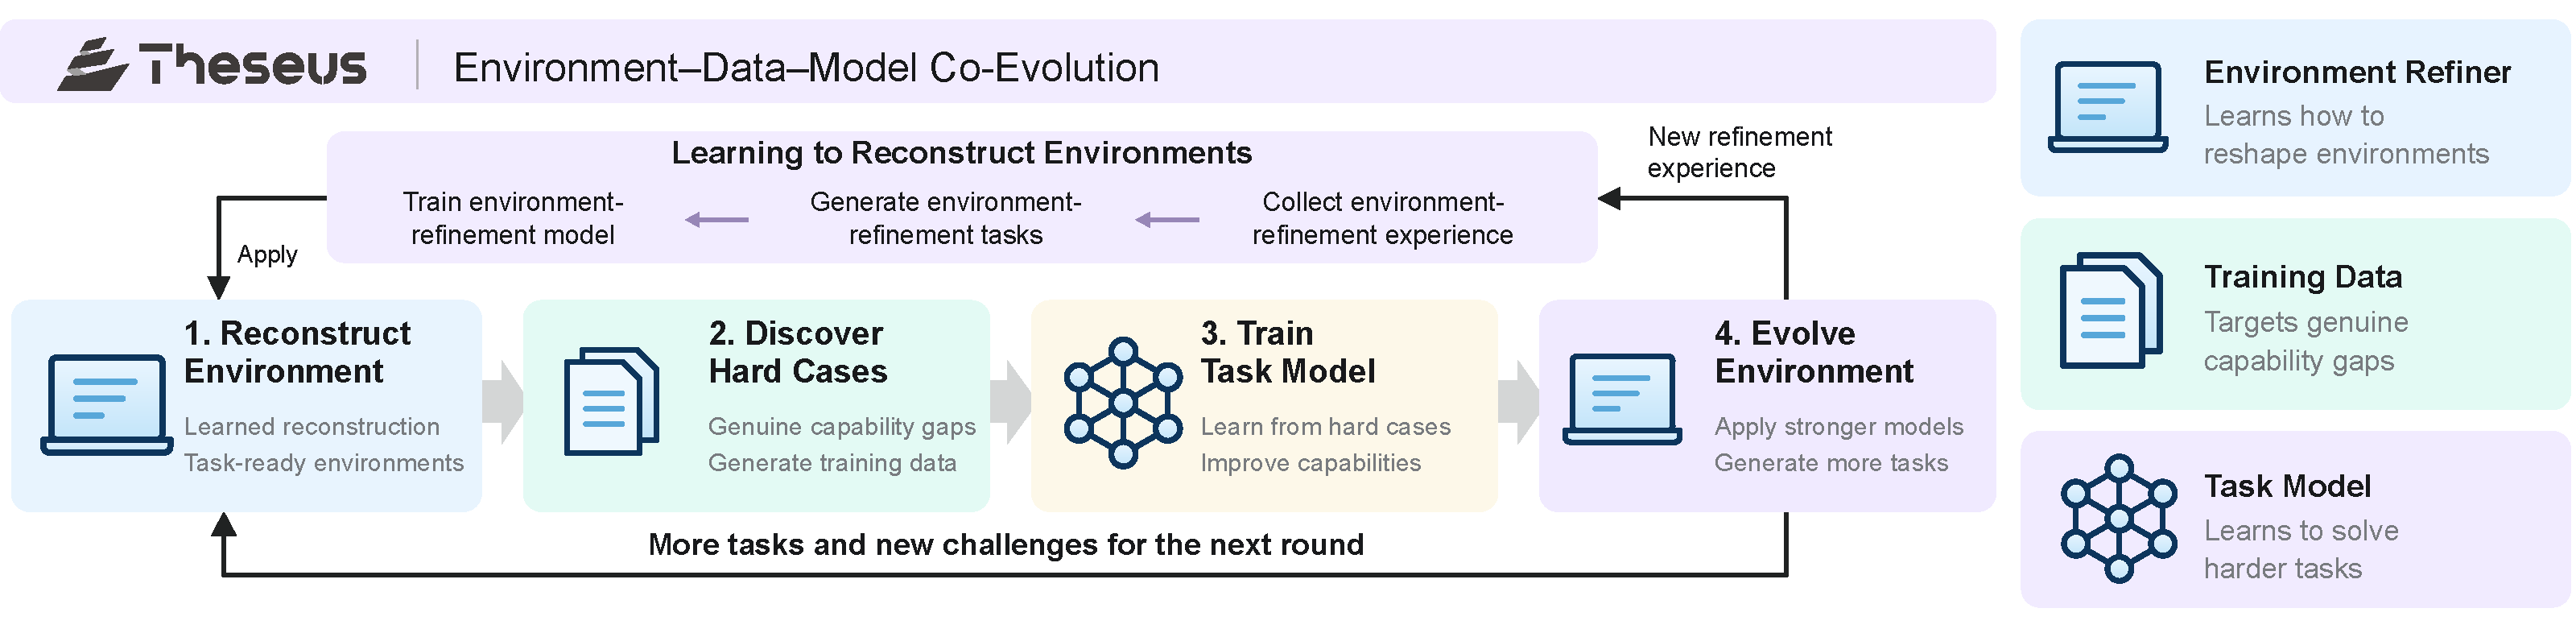
\includegraphics[width=\textwidth]{figures/Theseus.pdf}
    \caption{{Theseus's proposed four-stage co-evolution loop: reconstruct environments, uncover genuine capability gaps and generate training data, train task models, and iterate environments to produce more tasks. The upper loop learns an environment-refinement model from refinement experience and generated tasks, while successive iterations supply new experience for further refinement.}}
    \label{fig:bt_theseus}
\end{figure*}

{Theseus positions environment--data--model co-evolution as a path toward next-generation RSI intelligence. Its central premise is that environments make knowledge accessible and actions verifiable, task execution produces evidence for learning, and improved models expand the range of problems that can be explored. Under this vision, each round of work should contribute reusable capabilities to subsequent rounds, making real-world practice a continuing source of intelligence growth.} % \footnote{This case summarizes company-provided research and project materials current as of September 2026, including the working manuscript \emph{Hitting the Environment Wall: Evolving LLM Agent Workspaces for Recursive Self-Improvement}.}
%  progress should accumulate in the conditions that make future learning possible

{As shown in Figure~\ref{fig:bt_theseus}, Theseus realizes this vision in four steps. First, refinement experience is converted into environment-refinement tasks to train an environment-refinement model. Second, agents use reconstructed environments to identify genuine task-solving difficulties and generate targeted training data. Third, these data train the task model to improve its capabilities. Fourth, the stronger model supports further environment iteration and the generation of more tasks. Subsequent rounds yield both new task-training data and new environment-refinement experience, linking progress in solving tasks to progress in constructing the conditions for future learning.} % environment reconstruction becomes a learned capability: refinement experience is converted into 

{Early results provide an initial empirical basis for this direction in the workspace stage of the loop. A pilot with eight frontier model--harness configurations on 30 workspace tasks adapted from Workspace-Bench~\cite{tang2026workspacebench}, scored by 1,280 rubrics, first measured sensitivity to workspace quality: relative to a noise-laden workspace, a clean workspace raised pass rates by 21.7--51.6 percentage points across all eight configurations (Table~\ref{tab:theseus_results}a), suggesting that workspace state, rather than model capability alone, can bound agent performance. Building on this observation, a follow-up productivity study asked whether enriching the environment improves task performance while keeping the underlying model and harness fixed: five fixed model--harness pairings solved 30 tasks scored by 547 rubrics in total under a bare workspace and a reconstructed environment consisting of a Collection Map and an Event Log; the reconstructed environment raised aggregate rubric scores by 18.65--39.67 percentage points across all tested configurations (Table~\ref{tab:theseus_results}b), although a few tasks showed scope-creep regressions, where agents produced more extensive changes than the task required. The team has also completed training a reusable file-verification module. These early results mark the first steps of the co-evolution loop, and successive rounds will extend environment reconstruction, data generation, and model training into a sustained cycle of compounding improvement.}

%\wyk{Theseus's broader ambition is to make AI for Science a source of progress for future foundation models. Its project vision spans scientific frontiers including quantum computing, chemistry, controlled fusion, and brain science, where exploration can generate demanding tasks, testable hypotheses, and informative feedback. The intended relationship is reciprocal: stronger models advance scientific work, while scientific experience supplies knowledge and learning opportunities for subsequent models. Framed as an \emph{Evolution Model}, this agenda places sustained learning from practice at the center of model development and illustrates an environment-centered route toward RSI.}


\subsection{Lark: Building the Data Foundation for Reliable Enterprise-Level RSI}


Figure~\ref{fig:bt_lark} summarizes Lark's data-foundation loop. Lark approaches RSI from a prerequisite that is often overlooked: before an agent can improve itself, it needs a continuously evolving data substrate on which improvement can be grounded. In enterprise collaboration, documents, messages, meetings, and tasks continuously generate new information, while agents consume these data and produce new interaction traces. Lark therefore treats data production, quality evaluation, and failure attribution as the foundation of its RSI pipeline. The key objective is not merely to accumulate more data, but to ensure that each iteration has fresh experience to learn from, a reliable criterion for judging progress, and sufficiently fine-grained diagnostics to determine what should be changed.

\textbf{Enterprise Knowledge Graph.} A representative example is the construction and continual refinement of an enterprise knowledge graph. Information scattered across documents, messages, and meeting records is linked into entities, events, people, and temporal relations so that agents can answer questions requiring cross-source reasoning. Because graph errors directly propagate into downstream answers, graph construction is itself treated as an iterative data-quality problem. Lark addresses scalability through batched graph construction and delegated authorization checks, while continuously evaluating whether graph-based retrieval improves downstream question answering. In internal evaluations, it reports that human-rated task usability increased from 52\% to 65\%, while automated-evaluation usability increased from 47\% to 56\% when using its graph-based pipeline compared with the RAG-based baseline.

\begin{figure*}[!t]
    \centering
    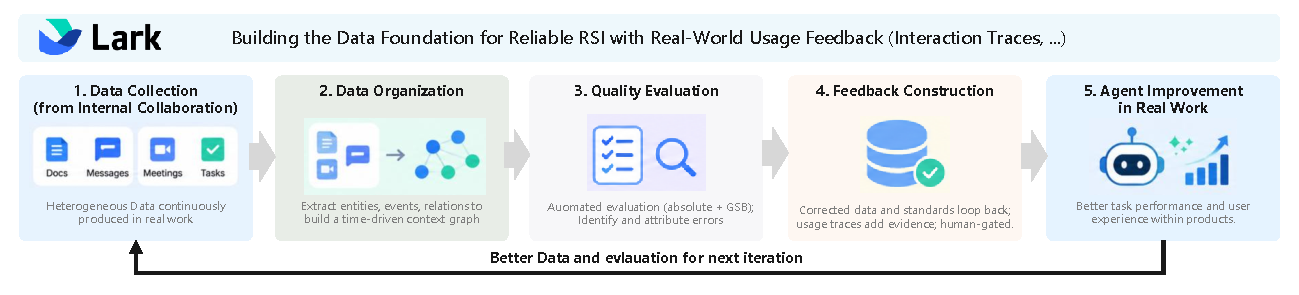
\includegraphics[width=\textwidth]{figures/Lark.pdf}
    \caption{Lark’s data-foundation loop for RSI, where collaboration data are continuously structured, evaluated, and refined into high-quality knowledge and training signals, while real-world agent usage feeds new evidence back into subsequent improvement cycles.}
    \label{fig:bt_lark}
\end{figure*}

\textbf{Automated Data-Quality Evaluation.} Another example is an automated data-quality evaluation system that serves as the measurement layer for subsequent improvement. Rather than relying entirely on expensive and inconsistent manual review, Lark first applies absolute judgments to identify clearly unusable outputs and then uses comparative GSB evaluation to determine whether a new system variant should be promoted. Importantly, evaluation is coupled with explicit failure attribution. Bad cases are categorized into issues (e.g., temporal inconsistency, distorted queries, or poor source quality), so that each failure maps to a concrete improvement direction. For example, time-sensitive questions are constrained by query-time filtering to avoid using future information, and low-quality synthetic queries are rewritten before re-entering the evaluation pipeline. The initial automated evaluator achieved approximately 84\% agreement with human judgments, where most disagreements arose because the automated evaluator was stricter than human reviewers, providing a concrete signal for subsequent calibration.

From an RSI perspective, the significance of these trials lies in the feedback structure they create for future agent improvement. Enterprise activity continuously produces new graph data and interaction traces, automated evaluation determines which outputs and data are reliable, error attribution identifies where the pipeline failed, and corrected data and evaluation standards then become inputs to later iterations. The resulting cycle turns production data from a passive resource into an evolving improvement substrate. At the same time, Lark's current practice remains deliberately human-gated: agents perform much of the repetitive data processing and evaluation, while humans retain responsibility for defining standards, reviewing critical samples, and approving important changes.

%The case of Lark illustrates a complementary industrial RSI principle to systems that directly self-modify prompts, tools, or source code: reliable self-improvement depends on first establishing a trustworthy data-and-evaluation foundation. Without these, an autonomous update loop may simply amplify noisy supervision or incorrect feedback. Lark's practice suggests that, particularly in enterprise settings, building this foundation can be a necessary intermediate step toward broader Agent RSI rather than an auxiliary data-engineering task.

\subsection{Xiaohongshu: Dual-Timescale RSI for Recommendation}


\begin{figure*}[t]
    \centering
    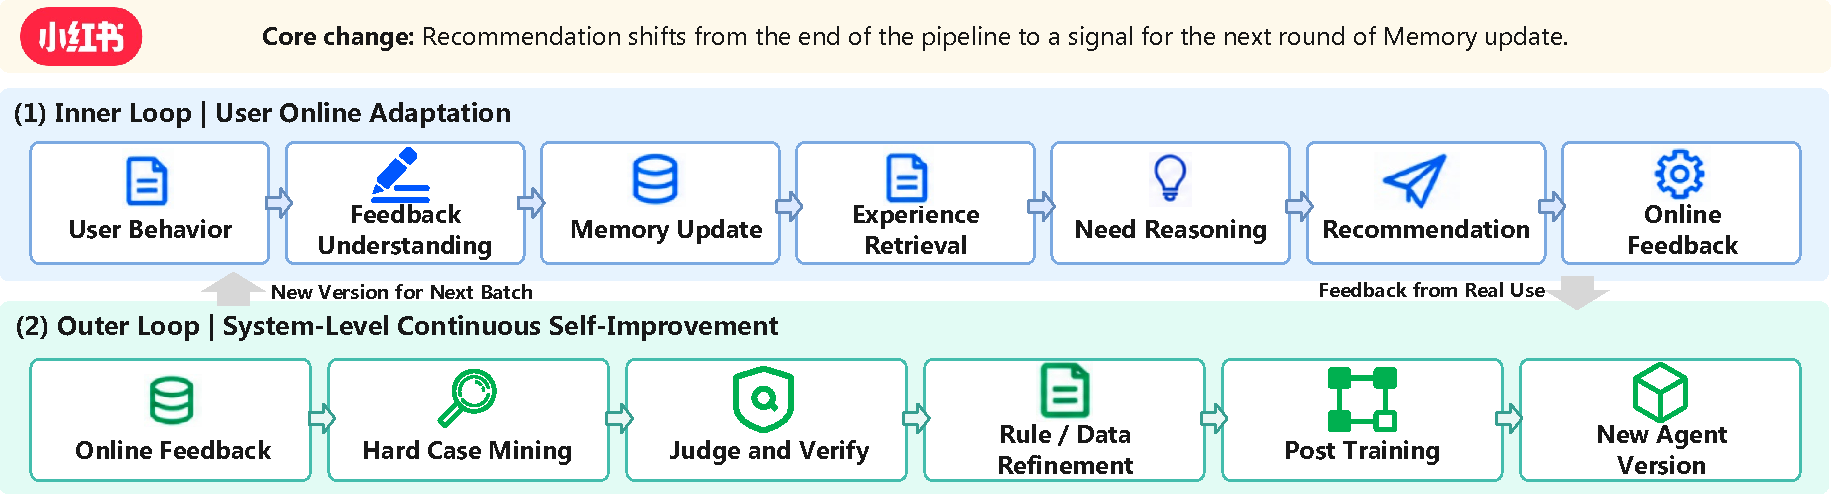
\includegraphics[width=\textwidth]{figures/xiaohongshu.pdf}
    \caption{Xiaohongshu’s dual-timescale RSI loop for recommendation. The Intent-Memory Agent (IMA) uses online behavioral feedback to update structured user memory and guide subsequent recommendations. At a slower timescale, hard cases undergo automated judging, human spot checks, and data reconstruction, supporting post-training updates that consolidate validated experience into agent parameters before redeployment.}
    \label{fig:bt_xiaohongshu}
\end{figure*}

% Table
\begin{table}[t]
    \centering
    \caption{Performance comparison between the online baseline
    and the RSI model at Xiaohongshu.}
    \label{tab:xiaohongshu_rsi}

    \small
    \setlength{\tabcolsep}{7pt}
    \renewcommand{\arraystretch}{1.2}

    \begin{tabular}{@{}llccc@{}}
        \toprule
        Module
        & Metric
        & \makecell{A: Online baseline}
        & \makecell{B: RSI model}
        & Improvement \\
        \midrule

        Discovery Feed
        & \texttt{score\_mean@16}
        & 2.211
        & 2.366
        & $+7.0\%$ \\

        Discovery Feed
        & \texttt{score\_median@16}
        & 1.587
        & 1.663
        & $+4.8\%$ \\

        \addlinespace[3pt]

        In-video Feed
        & \texttt{score\_mean@16}
        & \makecell{1.537 ($n=470$)}
        & \makecell{1.739 ($n=447$)}
        & $\approx +13.1\%$\textsuperscript{*} \\

        \bottomrule

    \end{tabular}
\end{table}

Xiaohongshu’s commercialization recommendation system explores feedback-driven self-improvement through an Intent-Memory Agent (IMA). Rather than treating user understanding as a one-off inference from historical behavior, IMA connects feedback interpretation, memory updating, experience retrieval, need reasoning, and recommendation into a continuous cycle. Subsequent clicks, dwell time, saves, searches, conversions, and negative feedback serve not only as new behavioral inputs, but also as observations against which earlier estimates of user state and intent are checked. These observations guide the addition, reinforcement, replacement, or decay of memory, as well as decisions to ignore uninformative evidence. The persistent improvement target is therefore the user representation that informs future recommendations, rather than only the current recommendation output.

\textbf{Structured Memory and Experience Reuse.} IMA organizes its intermediate state into three semantic layers: Content, describing the content topic; Who, representing the user’s state; and Need, specifying the inferred requirement. These layers also structure knowledge-base storage and retrieval, allowing historical experience to be recalled through content similarity, user-state similarity, or need similarity. This decomposition is intended to reduce retrieval errors caused by mixing distinct semantic factors in a single caption representation. It also enables subsequent feedback to correct particular state variables rather than indiscriminately rewriting the entire user profile.

\textbf{Fast Adaptation and Slower Capability Consolidation.} The system combines two complementary improvement cycles. At the user level, real-time feedback updates memory to accommodate changing interests and temporary needs. At the system level, high-value hard cases collected from online interactions undergo automated judging, human spot checks, rule correction, and training-data reconstruction. The resulting examples support post-training updates to IMA, and the updated agent returns to the recommendation pipeline. Long-tail experience can thus become immediately available through the knowledge base, while repeatedly validated patterns are gradually consolidated into model parameters. This dual-timescale design connects rapid, non-parametric adaptation with more persistent model-level learning.

\textbf{Reported Observations.} In the company-provided comparison, Discovery Feed’s score\_mean@16 increases from 2.211 to 2.366, a reported 7.0\% improvement, while score\_median@16 increases from 1.587 to 1.663, or 4.8\%. For the in-video feed, score\_mean@16 increases from 1.537 to 1.739, approximately 13.1\%. The latter result comes from a small offline evaluation with 470 baseline samples and 447 RSI-model samples. These findings should be interpreted as preliminary, company-reported ranking-score improvements; the supplied material does not establish corresponding gains in click-through or conversion rates.

The case illustrates an industrial RSI pattern in which recommendation outcomes become evidence for revising the system that produces subsequent recommendations. Online feedback corrects persistent user memory, while reviewed hard cases improve later agent versions through post-training. Its practical contribution is the coupling of immediate state correction, structured experience reuse, and longer-term capability consolidation, with human inspection retained in the training-data refinement process.




\subsection{Humanlaya: Delivery-Driven RSI for Data Quality Assurance}
\label{subsec:humanlaya}


Humanlaya provides training and evaluation data for foundation-model developers, with its production workflow centered on complex multi-file task packages consisting of task descriptions, input attachments, reference answers, scoring rubrics, and executable or procedural verification requirements. In such settings, quality failures are often subtle, where an individual artifact may appear correct in isolation while remaining inconsistent with the task specification, scoring logic, or downstream evaluation protocol. As task types and customer requirements evolve, repeatedly repairing individual defective samples is insufficient, and the quality-control system itself must learn from recurring failures. Humanlaya therefore treats its data-quality agents and their associated rules, prompts, few-shot examples, and skills as persistent improvement targets, including an inner loop and an outer loop, as shown in Figure~\ref{fig:bt_humanlaya}. % The production workflow contains two nested feedback loops.

\begin{figure*}[!t]
    \centering
    \includegraphics[width=\textwidth]{figures/Humanlaya.pdf}
    \caption{Humanlaya's delivery-driven RSI loop for data-quality assurance.}
    \label{fig:bt_humanlaya}
\end{figure*}

\textbf{The Data-Centric Inner Loop.} The inner loop operates within the current delivery batch and focuses on repairing the data being produced. Each task package first passes through a Quality Checker that inspects content quality and cross-component consistency, followed by a Refiner that repairs confirmed defects, and finally a Delivery Checker that verifies formatting, structure, and delivery constraints. Failed checks trigger repeated localization, revision, and re-verification before delivery. For example, if several independently gradable results are incorrectly merged into a single coarse rubric item, the checker may identify the rubric as insufficiently atomic and request restructuring before the package is accepted. This loop improves the current artifact, but by itself does not constitute persistent system improvement.

\textbf{The Improvement-Centric Outer Loop.} The outer loop operates across delivery batches and is the central RSI mechanism. After delivery, the system aggregates evidence like internal review, customer feedback, and downstream usage.  An agent analyzes these cases for recurrent causes and proposes versioned modifications to the quality-control system, including components like Refiner instructions, prompts, few-shot examples, and reusable skills. Candidate updates are evaluated on task packages that are not involved in producing the modification and are additionally reviewed by humans before promotion. Once approved, the new quality-system version replaces the previous one and is used for subsequent production batches. New tasks then generate new evidence, which again enters the next improvement cycle.

A representative case involved a three-page scanned PDF that the extraction tool failed to parse, causing the Quality Checker to mark the attachment as unusable. Manual review shows that the scan itself is clear, while the error comes from conflating extraction failure with poor document quality. The system therefore generates a new decision rule and few-shot examples to distinguish the two cases. After held-out validation and human review, the update is incorporated into the next system version and reused on future tasks.
The inner loop repairs the current task package, whereas the outer loop updates the method used to inspect and repair future packages. Humanlaya therefore represents a practical form of scaffold-level RSI driven by production feedback.

\textbf{Measured Improvement.} Humanlaya reports an internal comparison between V0 and V4 after four feedback-driven updates. Using the same base model, tools, and processing budget, both versions were evaluated on 600 task packages excluded from the update process. The rate of packages containing key defects after automated repair decreased from 9.0\% to 3.7\%, while average human handling time fell from 48 to 27 minutes per task. 

At the current stage, when model capabilities are still advancing rapidly, some tasks cannot yet be completed fully autonomously by agents. Humanlaya therefore provides a practical example of combining RSI with human oversight, where agents perform most of the self-improvement process, while humans provide partial ground truth, review, and final approval at critical stages, rather than allowing an unconstrained self-improvement loop.


\subsection{ModelBest: Zero-Human Industrial AI Engineering}

\begin{figure*}[t]
    \centering
    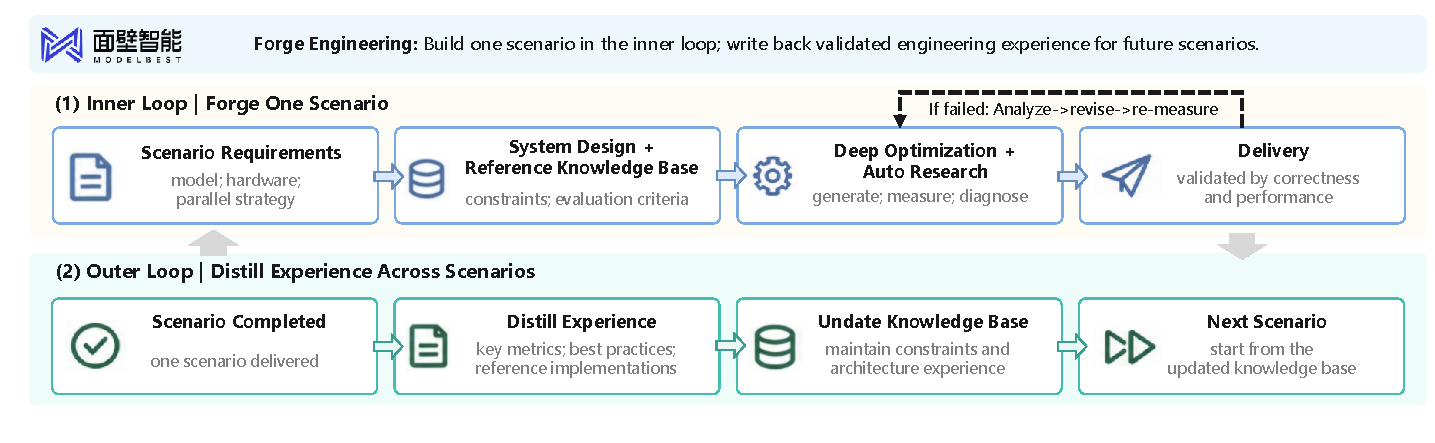
\includegraphics[width=\textwidth]{figures/ModelBest.pdf}
    \caption{
    ModelBest: Forge Engineering as a two-level RSI loop.}
    \label{fig:bt_modelbest}
\end{figure*}

ModelBest aims to advance RSI by automating AI engineering, based on the premise that \textit{AI engineering is likely to become autonomous earlier than open-ended AI research}. Engineering tasks (e.g., implementing training frameworks, optimizing kernels, configuring parallelism, running benchmarks) require substantial human effort but offer comparatively inexpensive, objective feedback through execution. To this end, to produce a production-ready implementation without human intervention, ModelBest proposes \textit{{Forge Engineering}}, an end-to-end paradigm in which an AI system takes a target model, hardware platform, and parallelization requirements as inputs, then builds, tests, and refines an implementation from an initially empty codebase. Figure~\ref{fig:bt_modelbest} shows how its within-project optimization and cross-project experience reuse form a two-level loop. %The goal is  within the engineering loop.

\textbf{The Industrial RSI Loop.} Within a target scenario, the system combines constrained architecture design with autonomous low-level optimization. Humans and AI maintain a knowledge base containing specifications, evaluation criteria, and accumulated engineering experience. The agent first uses this knowledge to establish a reasonable high-level architecture and constrain the search space. An AutoResearch loop then repeatedly generates implementations, measures correctness and performance, diagnoses failures, and repairs bottlenecks. Successful optimizations, including kernels such as GEMM and FlashAttention, are progressively integrated into the main execution path. This design keeps global architectural constraints stable while allowing aggressive autonomous optimization at the implementation level.

Across scenarios, successful and failed engineering experience is written back into the shared knowledge base. Performance measurements, effective optimization strategies, reference implementations, and failure rules from one project become starting knowledge for subsequent projects. The same engineering procedure can therefore be reused across different models, hardware platforms, and workloads. ModelBest reports applying the paradigm across pre-training frameworks, operator libraries, reinforcement-learning infrastructure, inference engines, fine-tuning, compression, quantization, and edge deployment on several hardware ecosystems.


\textbf{Measured Improvement.} Starting from an empty directory together with reference scripts and model specifications, ForgeTrain~\cite{forgetrain2026} generated a pre-training framework that matched Megatron-LM v0.15 within roughly 8 hours and reportedly surpassed it within 1.5–2.5 days, compared with an estimated 3–5 engineers working for 6–12 months for comparable manual development. Reported model FLOPs utilization increased from 40.1\% to 44.1\% for MiniCPM4-0.5B and from 47.0\% to 50.9\% for the 8B model. ForgeStencil~\cite{forgestencil} extends the same approach to scientific-computing kernels, with the company reporting 1.15–1.9× speedups over public state-of-the-art implementations and a median 1.41× end-to-end speedup.

%The case of ModelBest illustrates a distinct industrial RSI pattern to maximize autonomy where feedback is cheap, executable, and reversible, while retain explicit constraints at the architectural and evaluation boundaries. More importantly, the persistent improvement is not merely the optimized code produced in one run. Cross-project engineering experience, like successful strategies, failure modes, and reference implementations, is accumulated and reused to improve subsequent engineering loops. In this sense, Forge Engineering moves from autonomous code generation toward an engineering system whose accumulated experience increasingly shapes how future AI infrastructure is built.


\subsection{Tencent Hunyuan: Experience-Driven Self-Improvement}

\begin{figure*}[t]
    \centering
    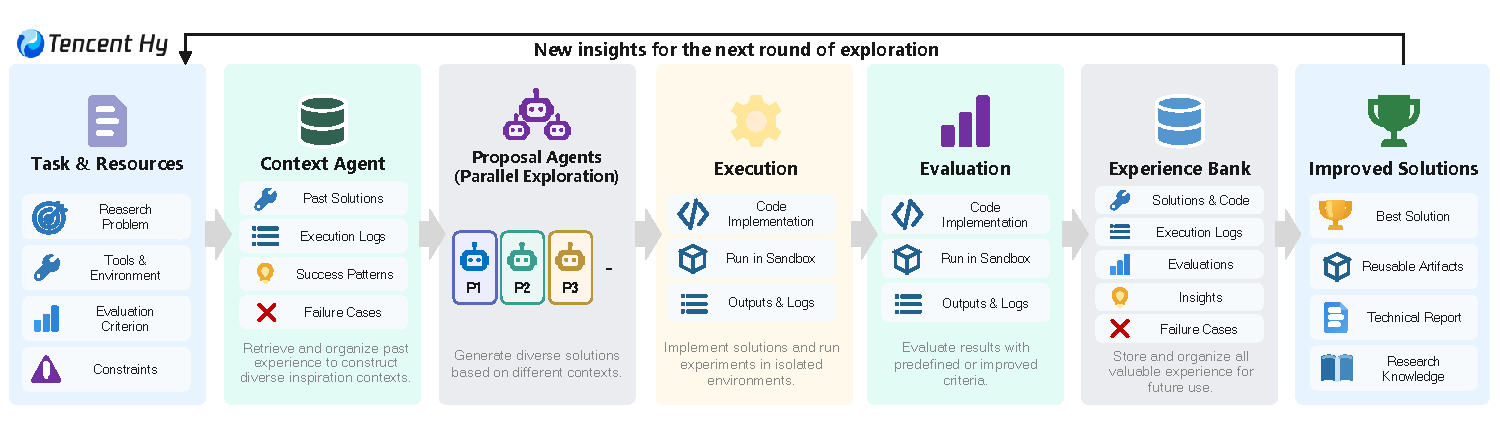
\includegraphics[width=\textwidth]{figures/Hy.pdf}
    \caption{Experience-driven self-improvement in Tencent Hunyuan Hyra. A Context Agent organizes prior experience to guide parallel solution proposals, which are executed in isolated environments and evaluated. The resulting code, execution logs, and evaluation feedback are retained in an Experience Bank to inform subsequent exploration and support evaluator refinement when needed.}
    \label{fig:bt_hunyuan}
\end{figure*}


Tencent Hunyuan's Hyra (Hunyuan Research Agent) explores RSI in performance-oriented research and engineering tasks. Figure~\ref{fig:bt_hunyuan} outlines its experience-driven search loop. Its design follows a deliberately lightweight philosophy: rather than encoding increasingly elaborate human-designed workflows, Hyra gives agents a broad solution space and repeatedly uses experimental evidence to guide subsequent search. Given a task, the system continues exploring until it decides to terminate or exhausts its resource budget, returning the best solution discovered during the process.

A central component is the Experience Bank, which retains substantially richer state (e.g., previous solution code, generated artifacts, execution logs, scores, and evaluator feedback) than a conventional textual memory. A Context Agent recombines this evidence into diverse inspiration contexts, while multiple Proposal Agents asynchronously consume these contexts, construct new solutions, and execute them in fresh isolated sandboxes. The resulting artifacts and evaluation outcomes are written back into the Experience Bank, allowing later proposals to directly reuse, combine, or avoid patterns discovered in earlier attempts.

Hyra further extends this idea to evaluation itself. For open-ended tasks where the initial evaluator is incomplete or becomes exploitable, accumulated search experience can be used to revise the evaluation mechanism—for example, by increasing its granularity, strengthening comparison baselines, or closing reward-hacking loopholes—before subsequent search continues under the improved criterion. This is particularly relevant to RSI because the persistent update is no longer limited to a better solution: the mechanism that determines which future solutions are considered improvements can also change.


\begin{table}[t]
    \centering
    \caption{Comparison of Recursive and hyra-1.0 on AI R\&D benchmarks.}
    \label{tab:hyra_benchmarks}
    \small
    \setlength{\tabcolsep}{5pt}
    \renewcommand{\arraystretch}{1.1}
    \renewcommand{\tabularxcolumn}[1]{m{#1}}

    \begin{tabularx}{\linewidth}{
        @{}
        >{\centering\arraybackslash}X
        >{\centering\arraybackslash}X
        >{\centering\arraybackslash}X
        c
        c
        @{}
    }
        \toprule
        \textbf{Benchmark}
        & \textbf{Task}
        & \textbf{Metric}
        & \textbf{Recursive}
        & \textbf{hyra-1.0} \\
        \midrule

        NanoChat Autoresearch~\cite{nanogpt_ar}
        & Model training
        & Validation BPB $\downarrow$
        & 0.9109
        & \textbf{0.9015} \\

        \addlinespace
        NanoGPT Speedrun~\cite{modded_nanogpt_2024}
        & Model training acceleration
        & Time to 3.28 loss $\downarrow$
        & 77.5\,s
        & \textbf{76.4\,s} \\

        \addlinespace
        SOL-ExecBench~\cite{lin2026solexecbench}
        & GPU kernel optimization
        & Mean SOL $\uparrow$
        & 0.754
        & \textbf{0.771}$^{\dagger}$ \\

        \bottomrule
    \end{tabularx}
\end{table}

\textbf{Measured Improvement.} As shown in Table~\ref{tab:hyra_benchmarks}, the released companion artifacts report improvements across both AI-for-AI and AI-for-Science tasks. For example, Hyra reports validation BPB of 0.9015 on nanochat AutoResearch~\cite{nanogpt_ar} compared with a cited previous best of 0.9109, 76.4 s on nanoGPT Speedrun~\cite{modded_nanogpt_2024} compared with 77.5 s, and 0.771 on SOL-ExecBench~\cite{lin2026solexecbench} compared with 0.754. As an industrial RSI practice, Hyra highlights the value of retaining executable experience rather than only final answers. %The repository also contains results in mathematical optimization, packing, compact neural architectures, and molecular docking, together with reproducible artifacts for several tasks. These results should nevertheless be interpreted as company-released evidence rather than independent replication.



%Its improvement process is built around persistent experimental evidence, parallel exploration, isolated execution, and adaptive evaluation. More broadly, the case suggests that practical RSI can emerge even without continual model-weight updates: substantial improvement may instead be accumulated in the research state and in the mechanisms used to generate and evaluate subsequent solutions.


\subsection{Agent-Native Research Lab: Verifiable Research Infrastructure for RSI}

\begin{figure*}[t]
    \centering
    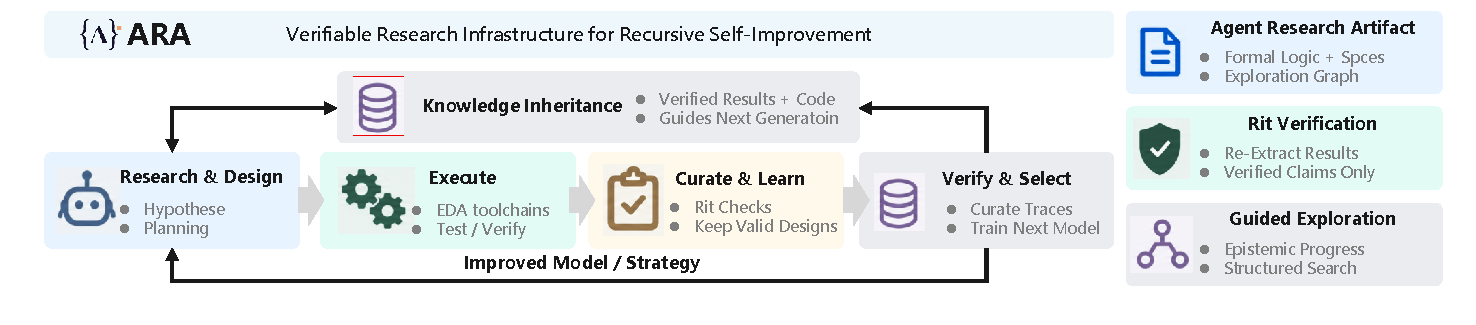
\includegraphics[width=\textwidth]{figures/ARA.pdf}
    \caption{Agent-Native Research Lab's agent-native RSI loop for verifiable engineering discovery, integrating guided exploration, deterministic verification, knowledge inheritance, and next-generation learning to support persistent improvement across research cycles.}
    \label{fig:bt_amber}
\end{figure*}

Achieving sustained recursive self-improvement requires more than increasingly autonomous research agents, while it also requires an infrastructure through which research experience can be reliably recorded, verified, inherited, and reused across generations. Agent-Native Research Lab focuses on this infrastructural layer, summarized in Figure~\ref{fig:bt_amber}. 

$\bullet$ \textbf{(1) Human-Centric vs. Agent-Native Research Artifact.} Conventional scientific papers are designed for human communication and would discard much of the operational state that autonomous agents need to continue previous work (e.g., failed experiments, intermediate evidence, executable specifications, and implementation details). For RSI, such information loss directly weakens cross-generation knowledge accumulation.

To address this, they propose Agent-Native Research Artifact (ARA) as an executable alternative to conventional scientific documentation. ARA jointly preserves formal scientific logic, executable code and specifications, the exploration graph of both successful and abandoned branches, and raw empirical evidence. Rather than inheriting only a polished final narrative, a successor agent can therefore inspect how a result was obtained, which alternatives failed, and which assumptions or parameters were actually used. The reported evaluation shows 93.7\% question-answering accuracy over prior work using ARA compared with 72.4\% using conventional papers, while RE-Bench reproduction success increases from 57.4\% to 64.4\%. The important RSI contribution is thus not merely better documentation, but a richer inheritance substrate for later research cycles.

$\bullet$ \textbf{(2) Deterministic Verification for Research Claims.} Additionally, as autonomous agents generate experiments and claims at machine speed, \textit{verification rather than generation becomes the main bottleneck}. Its rit protocol anchors empirical claims directly to execution traces, re-extracting reported results from logs, while analytical claims can be checked through formal verification systems such as Lean 4. Only claims that pass these machine-verifiable gates are admitted into the shared research state. This prevents hallucinated or incorrectly reported results from being recursively inherited and amplified by later generations. They also augment sparse outcome-based optimization with epistemic-progress guidance and structured priors derived from human scientific reasoning. Instead of rewarding only the final benchmark score, agents are encouraged to prefer experiments that reduce uncertainty and reveal useful structure in the problem. This is intended to improve research efficiency in large hypothesis spaces, where naive hill climbing can repeatedly exploit familiar parameters without producing deeper understanding.

\textbf{Measured Improvement.} These ideas are instantiated in silicon design, where the feedback loop is unusually fast and deterministic. Autonomous agents generate synthesizable SystemVerilog, construct testbenches, and propose microarchitectural modifications; candidates are then evaluated using industrial EDA tools for synthesis, place-and-route, timing analysis, and formal equivalence. Invalid designs are filtered automatically, while verified implementations, execution traces, failed branches, and superior power-performance-area trajectories are retained as training and research evidence for subsequent generations. On Chip-Bench, they report a Level-3 CPU optimization score of 5.8416, with a design that is 2.7\% faster and 21.5\% smaller in area than standard-agent baselines on the same model foundation while passing all 97 directed tests and 350 random differential programs.

%As an RSI best practice, the case of Agent-Native Research Lab highlights two requirements that are often missing from self-improving systems: high-fidelity inheritance and trustworthy promotion. The research artifact preserves enough state for later agents to build on both successes and failures, while deterministic verification controls which claims are allowed to enter the lineage. The lab further maintains authenticated generation lineage, strict holdout separation, and a frozen baseline to isolate the effect of the evolving research artifact. Multi-generation compounding under matched budgets is still an ongoing evaluation target, but the system provides a concrete infrastructure for measuring whether autonomous research improvements genuinely accumulate rather than merely producing isolated better outputs.






\iffalse
Achieving genuine recursive self-improvement requires an AI-native infrastructure engineered from first principles for autonomous AI scientists. 
Today, every convention carrying scientific knowledge arose around human cognitive limits. A paper is linear because human attention operates serially. It relies on prose because natural language provides shared communication without shared tooling. It runs a few thousand words to match a referee's finite reading time. Peer review anchors trust in personal reputation because manual re-execution is prohibitively expensive. These historical conventions form an interface built specifically for human biology. Autonomous agents operating in a recursive self-improvement loop represent an entirely different species of researcher, proposing, executing, verifying, and inheriting findings at machine speed. Forcing these agents to communicate through human-tailored documents creates severe friction. Genuine recursive progress demands a scientific infrastructure built natively for artificial intelligence: redesigning how research is recorded, verified, and compounded across cycles, while preserving the foundational principles of scientific inquiry.

Human civilization began accumulating wisdom only after developing language. Language provided the transmission protocol that allowed insights to compound across generations, preserving discoveries across lifetimes. In autonomous research, the protocol used to document knowledge serves as this exact primitive for compounding. Traditional scientific papers break this accumulation mechanism by discarding the operational history an agent needs to build on past cycles. On RE-Bench, failed runs consume 90.2\% of dollar costs with a median failed-to-success token ratio of 113x, yet traditional write-ups drop these dead ends entirely. On PaperBench, only 45.4\% of 8,921 reproduction requirements are fully specified. When an inheritance loop drops nine-tenths of its experimental history and leaves half of its parameters implicit, knowledge compounding collapses. The Agent-Native Research Artifact (ARA) defines an executable transmission protocol for machine agents across four interlocking layers: formal scientific logic, code with executable specifications, an exploration graph preserving abandoned branches, and raw empirical evidence. On this protocol, agents achieve 93.7\% question-answering accuracy on prior work compared to 72.4\% on papers, and lift RE-Bench reproduction success from 57.4\% to 64.4\%.

Trust requires an equally fundamental overhaul because autonomous agents generate claims orders of magnitude faster than conventional science can evaluate them. When an agent runs unsupervised for days, generation becomes trivial while verification becomes the defining bottleneck. Language models are probabilistic and routinely hallucinate findings. Without rigorous verification, agents accept fabricated metrics as true, building successive experiments on invalid premises. These errors compound across generations, spinning the agents into endless cycles of ungrounded iteration that squander compute. Auditing these claims through prose or secondary model judges fails because evaluating one probabilistic model with another preserves the underlying uncertainty. Automated research demands deterministic verification. The \texttt{rit} protocol anchors claims directly to machine checks: empirical figures are deterministically re-extracted from execution logs, while analytical propositions pass through formal verification kernels like Lean 4. Claims enter the shared knowledge base only after passing these automated gates. Establishing verification as a strict gate ensures agents iterate on reproducible findings, preventing error cascades and protecting compute resources.

Much of the wisdom guiding scientific discovery can be learned directly from human inquiry and its underlying philosophy. Centuries of human science show that breakthroughs require more than brute-force optimization against a sparse outcome score. An agent optimizing solely for a final benchmark score repeatedly overfits familiar parameters. Productive exploration relies on epistemic progress, a concept rooted in the philosophy of science where researchers track how each intermediate experiment reduces uncertainty about the physical world. In simulated physics environments, agents equipped with a continuous epistemic-progress signal uncover hidden physical laws where traditional optimization baselines stall. Human inquiry also contributes the philosophy of research taste: the heuristic discernment that identifies promising hypotheses early. Frameworks like Sci-Reasoning decode the decision paths of skilled human scientists into structured priors that agents can inherit. Autonomous systems can adopt these human heuristics to guide their search through vast hypothesis spaces.

We applied these techniques to silicon design because hardware engineering provides an exceptionally fast, deterministic domain to close the self-improvement loop. Our work extends beyond standard model pretraining into an active recursive self-improvement flywheel. In this framework, autonomous agents write synthesizable SystemVerilog modules, generate rigorous testbenches, and implement microarchitectural optimizations. Every proposed implementation directly confronts industrial EDA toolchains: logic synthesis via Yosys, place-and-route under nextpnr, static timing analysis through OpenSTA, and formal equivalence proofs with SymbiYosys. Circuits must satisfy cycle-accurate correctness, timing closure, and strict physical area bounds. The toolchain filters out invalid attempts and automatically compiles physically verified solutions and superior PPA (power, performance, area) trajectories into high-quality training corpora. Training successive model generations on these verifiable engineering traces enables the system to produce progressively superior hardware implementations and search strategies over time.

We evaluate this self-evolving system on Chip-Bench (https://chipbench.ai/), an open benchmark maintained by ARA Labs for AI chip engineering. Chip-Bench evaluates agents across two demanding tracks governed entirely by EDA toolchains with zero model grading: a three-level CPU generation track culminating in full PPA optimization, and a hill-climb track containing 20 optimization tasks across 6 layers of the silicon stack. Standard agent models struggle against these physical constraints, frequently breaking cycle-level functional equivalence or failing timing closure during aggressive microarchitectural edits. In contrast, our self-evolving system, integrating continuous epistemic-progress guidance and structured exploration graphs, consistently outperforms standard agent models across the optimization suite. On Level 3 CPU optimization, the guided system achieves the highest public optimization score of 5.8416, delivering a processor core 2.7\% faster with 21.5\% less area compared to standard agent baselines on the same model foundation, while passing all 97 directed tests and 350 random differential programs. Across the hill-climb optimization suite, the system establishes leading records on challenging sub-tasks, including arithmetic pipeline frequency scaling (scoring 1.060 against reference) and logic synthesis recipes. These empirical gains demonstrate how verifiable, closed-loop evolution enables automated systems to solve dense engineering challenges where raw model generation falters.

The scope of these empirical results remains specific. Each produced artifact is preserved, guides subsequent work cycles, and supports independent verification without relying on the producer's credibility. Demonstrating matched-budget compounding across multiple generations remains an ongoing effort. The evaluation machinery is operational: authenticated lineage envelopes bind each generation to its parent state, benchmark reporting enforces strict holdout separation, and a frozen baseline isolates the research artifact as the single mutable variable. These instruments provide the foundation needed to measure multi-generation compounding curves systematically.
\fi




\subsection{Frontis.AI: Enterprise Agent Evolution and Cross-Task Meta-Improvement}


\begin{figure*}[t]
    \centering
    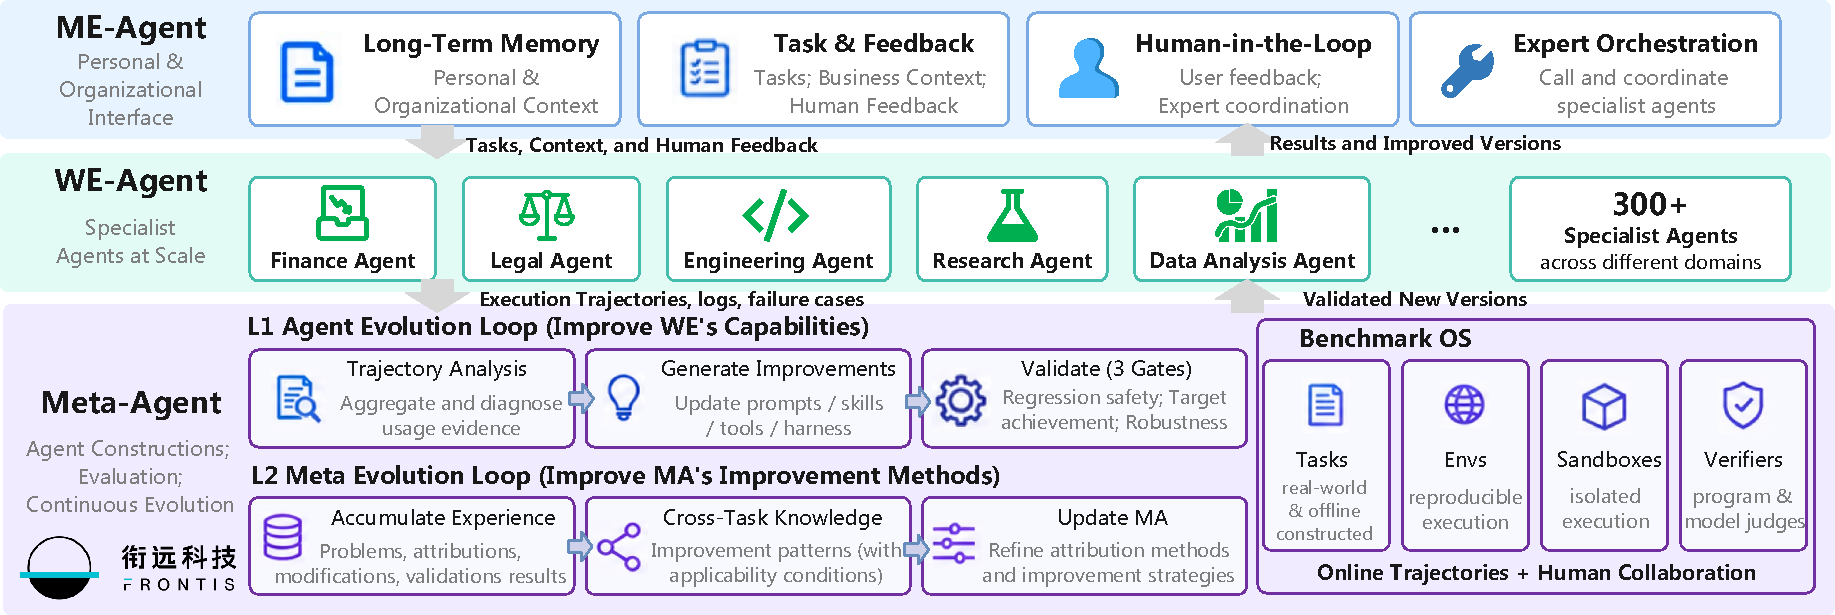
\includegraphics[width=\textwidth]{figures/frontis.pdf}
    \caption{Frontis Horizon’s ME–WE–MA architecture combines specialist-agent evolution and cross-task meta-improvement with shared evaluation and human-approved release.}
    \label{fig:bt_frontis}
\end{figure*}

Frontis Horizon provides an enterprise-owned infrastructure for improving both specialist agents and the methods used to improve them. Its ME–WE–MA architecture separates human interaction, contextual memory, and release approval (ME); task execution by more than 300 heterogeneous specialist agents across finance, legal, engineering, and human resources (WE); and agent construction, evaluation, and continuous evolution (MA). The central objective is to make improvement experience reusable across tasks rather than allowing it to remain isolated within individual agents.

\textbf{Business-Grounded Expert Evolution.} The platform’s Benchmark OS organizes enterprise tasks, reproducible environments, and verifiers into shared evaluation infrastructure. Programmatic checks are preferred, while semantic quality is assessed by model judges isolated from the evaluated agents. Given operational feedback, MA attributes failures to routing, execution mechanisms, or specialist capabilities, defines bounded improvement objectives and acceptance criteria, and obtains human confirmation before modifying prompts, skills, tools, or harnesses. Candidate versions are compared with their predecessors through three gates: regression safety, target achievement, and robustness in exceptional scenarios. Approved updates return to production with versioned test reports supporting audit and rollback.

\textbf{Cross-Task Meta-Improvement.} Beyond improving individual specialists, the platform retains each improvement episode’s problem context, diagnostic rationale, candidate modifications, validation results, and applicability conditions. Agent-specific experience supports subsequent versions, while transferable lessons inform MA’s diagnosis and improvement strategies on new tasks. Transfer requires adaptation and revalidation: a lesson about prioritizing real-time evidence, for example, still requires identifying authoritative sources and their temporal validity in the receiving task. This distinguishes learning to perform a business task from learning how to improve agents more effectively.

\textbf{Reported Outcomes.} Over two months, Frontis reports initiating 216 improvement tasks involving 117 specialist agents, of which 63 completed at least one full evolution cycle. Across 76 comparable tasks evaluated with the same evaluator, average scores increased from 5.25 to 5.87, with a median machine-processing time of 27.8 minutes per completed cycle. Separately, after accumulating meta-evolution experience from more than 100 tasks, the company reports approximately 20\% faster evolution on previously unseen internal test tasks relative to a process without cross-task experience. Its evaluation protocol distinguishes specialist performance from improvement efficiency by comparing identical initial agent versions and tracking iterations, time, token consumption, and regressions. These findings remain company-reported evidence rather than independent replication.

\textbf{Learning Improvement in Model Weights.} Frontis-MA1 separately explores training improvement capabilities into a 35B model. The supplied report records an MLE-Bench Lite score increase from 39.39\% to 60.61\% under a fixed harness, reaching 71.21\% with additional search. These results concern machine-learning and deep-learning engineering; extending the approach to learn directly from the platform’s enterprise-agent evolution trajectories remains future work.

The case illustrates a practical RSI pattern: retain not only improved agents, but also validated knowledge about how to improve them. Shared evaluation infrastructure, context-sensitive experience transfer, versioned updates, and human-controlled release provide the governance framework for this accumulation.




